\section{Project Management}
\label{sec:projectmanagement}

Group-07 manages the project through a defined team structure, a shared toolset,
a five-phase schedule and a repeatable workflow. The roles identify ownership,
the tools preserve review evidence and the workflow shows how a source file
becomes a verified database record. The same source files, normalization
outputs and final schema definition support both the report and the implementation.

\subsection{Group Structure and Roles}
\label{subsec:roles}

\begin{table}[H]
\centering
\caption{Group-07 roles and principal responsibilities}
\label{tab:roles}
\begin{tabular}{C{0.14\textwidth}L{0.26\textwidth}L{0.49\textwidth}}
\toprule
Roll ID & Name & Principal responsibilities \\
\midrule
24701026 & Sheikh Tawsif Bin Aftab & Team coordination, extraction, schema
implementation, deployment, maintenance and verification. \\
24701042 & Syed Mehraz Monwar & Documentation, report structure, drawing,
review and verification. \\
24701066 & Safwan Ahmed Rayed & Source collection, ER modelling, normalization
and documentation. \\
24701009 & Sanjida Mahi & Source review, normalization, final ERD and
verification. \\
\bottomrule
\end{tabular}
\end{table}

The responsibilities identify primary ownership rather than exclusive work.
Documentation and report work refer to the same shared deliverable while
modelling and verification receive more than one review. A change to the schema
or normalization therefore triggers checks in extraction, loading, queries and
the corresponding report explanation.

\subsection{Tools and Evidence}
\label{subsec:tools}

The tools support distinct parts of one workflow. Drive preserves the source
publications, Excalidraw records the design, Trello tracks work and Python and
SQLite produce the implementation. Git and LaTeX preserve the code and report
files. LLM was used for source-search assistance, transcription, wording review
and troubleshooting, while the retained sources and SQLite database remained
the basis for factual claims. Table~\ref{tab:tools} states these roles while
Figure~\ref{fig:project-tools} shows how the tools supported the main stages.

\begin{table}[H]
\centering
\caption{Tools used and the evidence each tool preserves}
\label{tab:tools}
\begin{tabular}{L{0.25\textwidth}L{0.64\textwidth}}
\toprule
Tool & Use in the project \\
\midrule
Google Drive & Original publications, team deliverables and report workspace. \\
Google Sheets & Source register and early inspection of candidate material. \\
Excalidraw & Collaborative ERD design and editable final diagram. \\
Trello & Sprint tasks, ownership and progress states. \\
Python and \texttt{openpyxl} & Extraction, preprocessing, normalization,
measurement generation and verification \cite{openpyxl}. \\
SQLite and SQL & Relational implementation, constraints and competency queries
\cite{sqlite}. \\
LLM & Source-search assistance, transcription, wording review and support with
LaTeX, Python and SQL troubleshooting; outputs were checked against project
files and the database. \\
Git and GitHub & Version history for the implementation and verification code. \\
LaTeX & Report text, citations, tables and reproducible diagrams. \\
\bottomrule
\end{tabular}
\end{table}

\begin{figure}[H]
\centering
\begin{tikzpicture}[
  stage/.style={draw=cublue,rounded corners=2pt,fill=cublue,
    text=white,text width=2.65cm,minimum height=1cm,align=center,
    font=\small\bfseries},
  tool/.style={draw=culine,rounded corners=2pt,fill=white,
    text width=2.65cm,minimum height=0.82cm,align=center,font=\small},
  lane/.style={draw=cuteal!55,rounded corners=3pt,fill=cugrey,inner sep=4pt},
  arr/.style={-{Stealth[length=2mm]},thick,draw=cuteal}
]
\node[stage] (source) at (0,0) {Sourcing and storage};
\node[tool,below=0.38cm of source] (drive) {Google Drive};
\node[tool,below=0.22cm of drive] (sheets) {Google Sheets};

\node[stage] (design) at (3.78,0) {Design and planning};
\node[tool,below=0.38cm of design] (excalidraw) {Excalidraw};
\node[tool,below=0.22cm of excalidraw] (trello) {Trello};

\node[stage] (implementation) at (7.56,0) {Implementation};
\node[tool,below=0.38cm of implementation] (python) {Python and \texttt{openpyxl}};
\node[tool,below=0.22cm of python] (sqlite) {SQLite and SQL};

\node[stage] (publishing) at (11.34,0) {Publishing};
\node[tool,below=0.38cm of publishing] (git) {Git and GitHub};
\node[tool,below=0.22cm of git] (latex) {LaTeX and Overleaf};

\node[tool,below=0.72cm of $(sheets)!0.5!(latex)$,text width=10.3cm]
  (llm) {LLM support: source search, transcription, wording review and
  troubleshooting; project files and SQLite remained the verification basis};

\begin{scope}[on background layer]
\node[lane,fit=(source)(drive)(sheets)] {};
\node[lane,fit=(design)(excalidraw)(trello)] {};
\node[lane,fit=(implementation)(python)(sqlite)] {};
\node[lane,fit=(publishing)(git)(latex)] {};
\end{scope}

\draw[arr] (source.east)--(design.west);
\draw[arr] (design.east)--(implementation.west);
\draw[arr] (implementation.east)--(publishing.west);
\end{tikzpicture}
\caption{Project tools grouped by their principal workflow stage. The arrows
show the main handoff order; the lower band records LLM as support across the
workflow rather than as project evidence.}
\label{fig:project-tools}
\end{figure}

\subsection{Time Period and Milestones}
\label{subsec:schedule}

Table~\ref{tab:schedule} gives the dated milestones,
Figure~\ref{fig:project-timeline} renders the same schedule and
Figure~\ref{fig:trello-workflow} preserves the team's task-board evidence.

\begin{table}[H]
\centering
\caption{Project time period and milestones}
\label{tab:schedule}
\begin{tabular}{L{0.20\textwidth}L{0.20\textwidth}L{0.50\textwidth}}
\toprule
Period & Phase & Main activity \\
\midrule
2--15 April & Discovery & Find and assess national and international sources. \\
16--29 April & Modelling & Identify entities, attributes, relationships and
candidate keys. \\
30 April--20 May & Extraction & Build source-specific extraction and record
layout problems. \\
21 May--10 June & Normalization & Reshape, reconcile and normalize selected
records. \\
11 June--20 August & Verification and reporting & Build and test the database,
revise the final ERD and prepare the report. \\
\bottomrule
\end{tabular}
\end{table}

\begin{figure}[H]
\centering
\begin{tikzpicture}[x=1cm,y=1cm,font=\sffamily\scriptsize]
  \def\gGut{3.62}      % gutter width for the task and date column
  \def\gDay{0.0780}    % centimetres per calendar day
  \def\gRow{0.95}      % lane height
  \def\gRight{15.4757} % right edge, 31 August
  \def\gBot{-7.90}     % bottom edge, eighth lane

  \node[anchor=west,font=\sffamily\bfseries\small,text=cublue] at (0,1.98)
    {Project schedule};
  \node[anchor=west,text=black!55] at (0,1.58)
    {Group 07 environment sector, 2 April to 20 August};

  \fill[cuteal!18]  ({\gGut+1*\gDay},0.52)    rectangle ({\gGut+28.5*\gDay},1.18);
  \fill[cuamber!18] ({\gGut+28.5*\gDay},0.52) rectangle ({\gGut+70.5*\gDay},1.18);
  \fill[cublue!18]  ({\gGut+70.5*\gDay},0.52) rectangle ({\gGut+141*\gDay},1.18);
  \node[text=cuteal!75!black]  at ({\gGut+14.75*\gDay},0.85)  {Sprint 1};
  \node[text=cuamber!75!black] at ({\gGut+49.5*\gDay},0.85)   {Sprint 2};
  \node[text=cublue!85!black]  at ({\gGut+105.75*\gDay},0.85) {Sprint 3};

  \fill[culine!45] (0,-0.30) rectangle (\gRight,0.40);
  \node[anchor=east,font=\sffamily\bfseries,text=cublue]
    at ({\gGut-0.17},0.05) {Task and dates};
  \foreach \c/\m in {15/April,45.5/May,76/June,106.5/July,137/August} {
    \node[font=\sffamily\bfseries,text=cublue] at ({\gGut+\c*\gDay},0.05) {\m};
  }

  \foreach \i in {2,4,6,8} {
    \fill[cugrey] (0,{-0.30-(\i-1)*\gRow}) rectangle (\gRight,{-0.30-\i*\gRow});
  }
  \foreach \d in {0,30,61,91,122,152} {
    \draw[culine] ({\gGut+\d*\gDay},0.40) -- ({\gGut+\d*\gDay},\gBot);
  }
  \foreach \i in {0,1,2,3,4,5,6,7,8} {
    \draw[culine] (0,{-0.30-\i*\gRow}) -- (\gRight,{-0.30-\i*\gRow});
  }
  \draw[culine] (0,0.40) rectangle (\gRight,\gBot);

  \foreach \i/\s/\e/\col in {%
    1/1/14/{cuteal!70},
    2/1/28/{cuteal!48},
    3/15/70/{cuamber!45},
    4/29/49/{cuamber!78},
    5/29/70/{cuamber!58},
    6/50/70/{cuamber!78},
    7/71/141/{cublue!62},
    8/71/141/{cublue!40}%
  } {
    \fill[\col,rounded corners=1.4pt]
      ({\gGut+\s*\gDay},{-0.30-(\i-0.5)*\gRow-0.20}) rectangle
      ({\gGut+\e*\gDay},{-0.30-(\i-0.5)*\gRow+0.20});
  }

  \foreach \i/\task/\dates in {%
    1/{Discover sources}/{2--15 April},
    2/{Verify and select sources}/{2--29 April},
    3/{Model and refine ERD}/{16 April--10 June},
    4/{Extract source blocks}/{30 April--20 May},
    5/{Clean and reconcile}/{30 April--10 June},
    6/{Normalize records}/{21 May--10 June},
    7/{Implement and test SQLite}/{11 June--20 August},
    8/{Draft and review report}/{11 June--20 August}%
  } {
    \node[anchor=east,text=black!85]
      at ({\gGut-0.17},{-0.30-(\i-0.5)*\gRow+0.20}) {\task};
    \node[anchor=east,font=\sffamily\tiny,text=black!50]
      at ({\gGut-0.17},{-0.30-(\i-0.5)*\gRow-0.22}) {\dates};
  }

  \draw[cublue,dashed,line width=0.4pt]
    ({\gGut+141*\gDay},-0.30) -- ({\gGut+141*\gDay},{\gBot-0.16});
  \node[anchor=north,font=\sffamily\tiny,text=cublue]
    at ({\gGut+141*\gDay},{\gBot-0.18}) {20 August};
\end{tikzpicture}
\caption{Full project Gantt chart. Lane dates follow the verified schedule of
Table~\ref{tab:schedule}; the sprint band above the calendar shows which
increment owns each lane, and the overlapping modelling, cleaning and reporting
lanes record concurrent work rather than a daily task log. Source: this LaTeX
code.}
\label{fig:project-timeline}
\end{figure}

\begin{figure}[H]
\centering
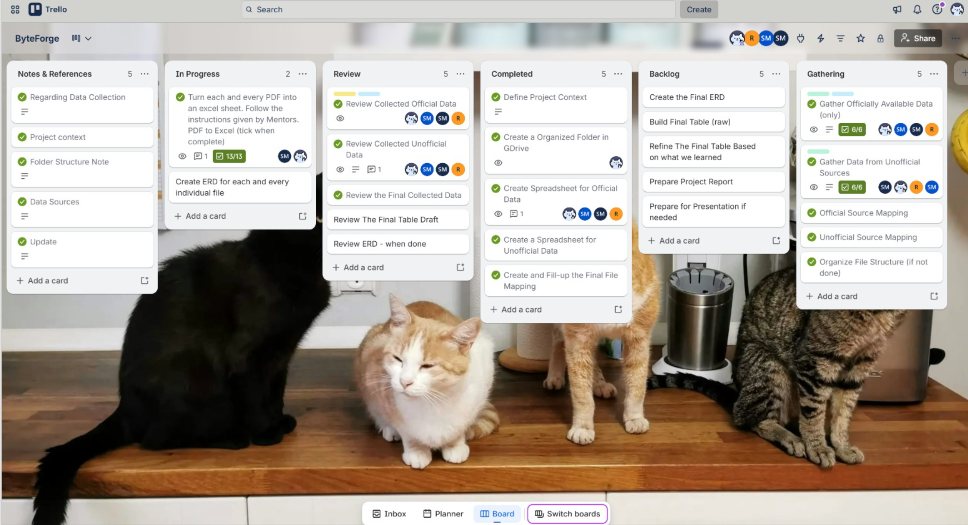
\includegraphics[width=0.84\textwidth]{Trello workflow.png}
\caption{Group-07 Trello board used to track sprint work. This is a screenshot
of the team's own board rather than a generated illustration.}
\label{fig:trello-workflow}
\end{figure}

\subsection{Workflow}
\label{subsec:workflow}

The workflow preserves original files, transforms copies through explicit
stages and verifies the database before its measurements enter the report.
Figure~\ref{fig:pipeline} shows the decision point between successful
verification and further correction. A failed key, row-count, integrity or
competency check sends the affected data, schema or query back for correction.
The process reaches report generation only after the required checks pass;
completing the database load alone is not sufficient verification.

\begin{figure}[H]
\centering
\begin{tikzpicture}[
  node distance=0.55cm,
  stage/.style={rectangle,rounded corners,draw=cublue,fill=cugrey,
    text width=2.25cm,minimum height=1cm,align=center,font=\small},
  decision/.style={diamond,draw=cuteal,fill=white,aspect=2.0,align=center,
    font=\small},
  arr/.style={-{Stealth[length=2mm]},draw=cuteal,thick}
]
\node[stage] (source) {Preserve source};
\node[stage,right=of source] (select) {Verify and select};
\node[stage,right=of select] (extract) {Extract blocks};
\node[stage,below=0.8cm of extract] (clean) {Clean and reconcile};
\node[stage,left=of clean] (normal) {Normalize};
\node[stage,left=of normal] (load) {Load SQLite};
\node[stage,below=0.8cm of load] (verify) {Test and review};
\node[decision,right=0.8cm of verify] (pass) {All checks pass?};
\node[stage,right=0.8cm of pass] (report) {Generate report evidence};
\node[stage,below=0.9cm of pass] (fix) {Correct data, schema or query};
\draw[arr] (source)--(select);
\draw[arr] (select)--(extract);
\draw[arr] (extract)--(clean);
\draw[arr] (clean)--(normal);
\draw[arr] (normal)--(load);
\draw[arr] (load)--(verify);
\draw[arr] (verify)--(pass);
\draw[arr] (pass)--node[above,font=\scriptsize]{yes}(report);
\draw[arr] (pass)--node[right,font=\scriptsize]{no}(fix);
\draw[arr,dashed] (fix.south) |- ($(fix.south)+(0,-0.45cm)$) -| (clean.south);
\end{tikzpicture}
\caption{Workflow from source publication to verified report output.}
\label{fig:pipeline}
\end{figure}
